\documentclass{beamer}
\usepackage{amsfonts}
\usepackage{amsmath}
\usepackage{times}
\usepackage{mathrsfs}
\usepackage{extarrows}
\usepackage{bbm} 
\setbeamercolor{footcolor}{fg=blue!100} % 设置字体和背景颜色
\setbeamertemplate{headline}{%
  \leavevmode%
  \hbox{%
    \hskip228pt
    \begin{beamercolorbox}[wd=.126\paperwidth,ht=2.25ex,dp=1ex,right]{footcolor}%      
       \textcolor[rgb]{0,0.168,0.376}{Slide \insertframenumber{} }
    \end{beamercolorbox}}%
  \vskip-19pt%
}

\setbeamertemplate{frametitle}
{
\vspace{30pt}\textcolor[rgb]{0,0.168,0.376}{\insertframetitle}
}

 
\pgfdeclareimage[height=0.61cm]{university-logo}{logo.png}  
\logo{\pgfuseimage{university-logo}{\vspace{244pt}}} 
\title{\textcolor[rgb]{0,0.168,0.376}{VV286 RC1}}
\author{JIANG Yicheng}
\begin{document}

\begin{frame}
\titlepage
\end{frame}


\begin{frame}
\frametitle{Separable Equations}
\begin{block}{Initial Value Problem (I.V.P.)}
$f$ is continuous in an interval $I_x\subset \mathbb{R}$; $g$ is continuous in an interval $I_y\subset \mathbb{R}$; $\xi\in I_x, \eta\in I_y$ 
$$\dfrac{dy}{dx}=f(x)g(y),\hspace{9mm}y(\xi)=\eta$$
\end{block}


\end{frame}
\begin{frame}
\begin{block}{Solution}
\begin{enumerate}
\item $g(\eta)\neq0$


$$\int_{\eta}^y\dfrac{ds}{g(s)}=\int_{\xi}^xf(t)dt\hspace{10mm} \text{(Unique solution)}$$
\item $g(\eta)=0$
\begin{enumerate}
\item Obvious solution
$$y(x)=\eta$$
\item Check $$\int_{\eta}^y\dfrac{ds}{g(s)}$$
in a small neighbourhood of $\eta$
\end{enumerate}
\end{enumerate}
\end{block}
\end{frame}


\begin{frame}
\begin{block}{Example}
$$\dfrac{dy}{dx}=x^4y+x^4y^4, \hspace{9mm}y(0)=1$$
$$y(0)=0?\,\,\,y(0)=-\dfrac{1}{2}?\,\,\,y(0)=-1?\,\,\,y(0)=-2?$$

\end{block}
\end{frame}

\begin{frame}
\begin{block}{Solution}
\begin{align*}
\int x^4dx&=\int \dfrac{1}{y+y^4}dy\\
\dfrac{1}{5}x^5&=\int \dfrac{1}{y}-\dfrac{y^2}{1+y^3}dy\\
\dfrac{1}{5}x^5&=\ln |y|-\dfrac{1}{3}\ln |1+y^3|+C\\
e^{3x^5/5}&=C\Bigg|\dfrac{y^3}{1+y^3}\Bigg|\\
\end{align*}
$$C=2\hspace{2mm}(y(0)=1);C=\dfrac{7}{8}\hspace{2mm}(y(0)=-2);C=7\hspace{2mm}(y(0)=-\dfrac{1}{2})$$
\end{block}
\end{frame}

\begin{frame}
\begin{block}{Equilibrium solution}
$$x_{equi}(t)=constant$$
\end{block}

\begin{block}{Steady-state solution}
$$x_{ss}(t)=\lim_{t\rightarrow\infty}x(t)$$
\end{block}

\begin{block}{Transient solution}
$$x(t)-x_{ss}$$
\end{block}
\end{frame}


\begin{frame}
\frametitle{Linear Equations}
A general linear, first-order ODE on an open interval $I\in\mathbb{R}$
$$a_1(x)y'+a_0(x)y=f(x),\hspace{3mm}x\in I $$
where $a_0,a_1,f$ is continuous, real-valued functions on $I$.
\end{frame}

\begin{frame}
\begin{block}{Solution}
$$y_{\text{inhom}}=y_{\text{part}}+y_{\text{hom}}$$
where 
$y_{\text{hom}}$ is the (general) solution of $a_1(x)y'+a_0(x)y=0$
\end{block}
\begin{block}{How to find a $y_{\text{part}}$?}
\end{block}
\end{frame}

\begin{frame}
\begin{block}{Variation of Parameters}
Set $y_{\text{inhom}}=c(x)y_{\text{hom}}(x)$, then
$$a_1(x)c'(x)y_{\text{hom}}(x)+\underbrace{a_1(x)c(x)y'_{\text{hom}}(x)+a_0(x)c(x)y_{\text{hom}}(x)}_{=0}=f(x)$$
solve $c(x)$.
\end{block}
\end{frame}

\begin{frame}
\begin{block}{Duhamel's Principle}
Let $I\subset\mathbb{R}$ be an open interval, $x_0\in\overline{I}$, and $a_0,a_1,f$ continuous, real-valued functions on $\overline{I}$, where $a_1(x)\neq0$ for all $x\in\overline{I}$. Let $y_{\xi}$ solve the initial value problem
$$a_1(x)y'+a_0(x)y=0,\hspace{3mm}y_{\xi}(\xi)=\dfrac{1}{a_1(\xi)}$$
for $x\in\overline{I}$. Then
$$y(x)=\int_{x_0}^xf(\xi)y_{\xi}(x)d\xi$$
solves
$$a_1(x)y'+a_0(x)y=f(x),\hspace{3mm}y(x_0)=0$$
\end{block}
\begin{block}{}
(Choose $c(\xi)$ which leads to $y_{\xi}(\xi)=c(\xi)y_{hom}(\xi)=\dfrac{1}{a_1(\xi)}$.)
\end{block}
\end{frame}

\begin{frame}
\begin{block}{Example}
$$\dfrac{dy}{dx}=3y+x$$
\end{block}
\end{frame}

\begin{frame}
\begin{block}{Solution}
\begin{enumerate}
\item $\dfrac{dy}{dx}-3y=0\Rightarrow y_{\text{hom}}=c\cdot e^{3x}$
\item Set $y_{\text{part}}=c(x)e^{3x}$, then $c'(x)e^{3x}=x$. So
\begin{align*}
c(x)&=\int xe^{-3x}dx=-\dfrac{1}{3}\int xd(e^{-3x})\\
&=-\dfrac{1}{3}\Big(xe^{-3x}-\int e^{-3x}dx\Big)\\
&=-\dfrac{1}{3}xe^{-3x}-\dfrac{1}{9}e^{-3x}
\end{align*}
Finally, $y=c\cdot e^{3x}-\dfrac{1}{3}x-\dfrac{1}{9}$
\end{enumerate}
\end{block}
\end{frame}

\begin{frame}
\frametitle{Transformable Equations}
\begin{block}{$y'=f(ax+by+c);b\neq0$}
$$u(x)=ax+by(x)+c$$
\end{block}
\begin{block}{$y'=f(y/x)$}
$$u(x)=\dfrac{y(x)}{x}$$
\end{block}
\end{frame}

\begin{frame}
\begin{block}{$y'=f\Big(\dfrac{a_1x+b_1y+c_1}{a_2x+b_2y+c_2}\Big)$}
$$u(x)=a_1x+b_1y(x)+c_1,v(x)=a_2x+b_2y(x)+c_2$$
$$x=\dfrac{b_2(u-c_1)-b_1(v-c_2)}{a_1b_2-a_2b_1}$$
$$\dfrac{du}{dv}=\dfrac{du}{dx}\cdot\dfrac{dx}{dv}=(a_1+b_1\dfrac{dy}{dx})\dfrac{b_2(du/dv)-b_1}{a_1b_2-a_2b_1}$$
$$\dfrac{du}{dv}=(a_1+b_1f\Big(\dfrac{u}{v}\Big))\dfrac{b_2(du/dv)-b_1}{a_1b_2-a_2b_1}$$
$$\dfrac{du}{dv}=b_2g\Big(\dfrac{u}{v}\Big)\dfrac{du}{dv}-b_1g\Big(\dfrac{u}{v}\Big)$$
$$\dfrac{du}{dv}=h\Big(\dfrac{u}{v}\Big)$$
\end{block}
\end{frame}

\begin{frame}
\begin{block}{Example}
$$y'=\dfrac{x-y}{x+y}$$
\end{block}
\end{frame}

\begin{frame}
\begin{block}{Solution}
Set $u(x)=\dfrac{y(x)}{x}$, then $\dfrac{1-u}{1+u}=y'=u'x+u$. So
$$\int \dfrac{1+u}{1-2u-u^2}du=\int \dfrac{1}{x}dx$$
$$\ln(u+1+\sqrt{2})+\ln(u+1-\sqrt{2})=-2\ln x+C$$
$$(y/x+(1+\sqrt{2}))(y/x+(1-\sqrt{2}))=\dfrac{C}{x^2}$$
$$y^2+2xy-x^2=C$$
$$y=-x\pm\sqrt{2x^2-C}$$
\end{block}
\end{frame}

\begin{frame}
\begin{block}{$y'+gy+hy^{\alpha}=0,\alpha\neq1$ (Bernoulli's equation)}
$$u(x)=(y(x))^{1-\alpha}$$
\begin{align*}
y'+gy+hy^\alpha=0&\Rightarrow (1-\alpha)y^{-\alpha}y'+(1-\alpha)gy^{1-\alpha}+(1-\alpha)h=0\\
&\Rightarrow (y^{1-\alpha})'+(1-\alpha)gy^{1-\alpha}+(1-\alpha)h=0\\
&\Rightarrow u'+(1-\alpha)gu+(1-\alpha)h=0\\
\end{align*}
\end{block}

\end{frame}

\begin{frame}
We assume $y(x)>0$ for all $x\in I$ and each strictly positive solution $u(x)$ can yield a strictly positive solution
$$y_+(x)=(u(x))^{1/(1-\alpha)}$$
\begin{block}{Note}
\begin{enumerate}
\item $\alpha>0$, $y=0$
\item $\alpha\in\mathbb{Z}, \alpha\equiv1(\text{mod 2})$, $y_-=-y_+$
\item $\alpha\in\mathbb{Z}, \alpha\equiv0(\text{mod 2})$, $y_-=-|u(x)|^{1/{(1-\alpha)}}$
\end{enumerate}
\end{block}
\end{frame}

\begin{frame}
\begin{block}{$y'+gy+hy^2=k$ (Ricatti's equation)}
\begin{enumerate}
\item Guess or given a solution $\phi$
\item For other solution $y$, set $u=y-\phi$, then
\begin{align*}
&\left\{
\begin{aligned}
y'+gy+hy^2=k\\
\phi'+g\phi+h\phi^2=k\\
\end{aligned}
\right.\\\Rightarrow & (y'-\phi')+g(y-\phi)+h(y-\phi)(y+\phi)=0\\
\Rightarrow&u'+gu+hu(u+2\phi)=0\\
\Rightarrow&u'+(g+2\phi h)u+hu^2=0
\end{align*}
\end{enumerate}
\end{block}
\end{frame}

\begin{frame}
\begin{block}{Example}
$$\dfrac{dy}{dx}=x^4y+x^4y^4, \hspace{9mm}y(0)=1$$
\end{block}
\end{frame}

\begin{frame}
\begin{block}{Solution}
$y(x)=0$ is not a solution.
$$y'-x^4y-x^4y^4=0\xLongrightarrow{\cdot (-3y^{-4})}(y^{-3})'+3x^4(y^{-3})+3x^4=0$$
Set $u=y^{-3}$, then $y=u^{-1/3}$.
$$u'+3x^4u=0\Rightarrow u_{\text{hom}}=c\cdot e^{-\frac{3}{5}x^5}$$
Set $u_{\text{part}}=c(x)\cdot e^{-\frac{3}{5}x^5}$, then 
$$c'(x)=-3x^4e^{\frac{3}{5}x^5}\Rightarrow c(x)=-e^{\frac{3}{5}x^5}$$
So $u(x)=c\cdot e^{-\frac{3}{5}x^5}-1$. Since $y(0)=1$, 
$$y=\dfrac{1}{\sqrt[3]{2e^{-3x^5/5}-1}}$$
\end{block}
\end{frame}

\begin{frame}
\frametitle{$h(x,y)y'+g(x,y)=0$}
\begin{block}{Another view}
$$h(x,y)y'+g(x,y)=0\Rightarrow\langle\begin{pmatrix}
1\\
y'
\end{pmatrix},\begin{pmatrix}
g(x,y)\\
h(x,y)
\end{pmatrix}\rangle=0$$
$\begin{pmatrix}
1\\
y'
\end{pmatrix}$: tangent vector of integral curve

\end{block}
\begin{block}{}
Integral curve is perpendicular to the vector field
$$F^{\perp}:\mathbb{R}^2\mapsto\mathbb{R}^2,\hspace{3mm}F^{\perp}(x,y)=\begin{pmatrix}
g(x,y)\\
h(x,y)
\end{pmatrix} $$
\end{block}
\end{frame}

\begin{frame}
\begin{block}{Equipotential Line}
Solution is $U(x,y)$=constant, where $U:\mathbb{R}^2\mapsto\mathbb{R}$ is a potential function of the conservation vector field

\end{block}
\begin{block}{What do we need to do?}
Find a potential function $U(x,y)$ whose gradient at each point is parallel to the vector $\begin{pmatrix}
g(x,y)\\h(x,y)
\end{pmatrix}$ i.e.
$$\nabla U(x,y)=M(x,y)\cdot F^{\perp}(x,y)$$
\end{block}
\end{frame}

\begin{frame}
\frametitle{Integrating factors (Euler Multipliers)}
Let $g,h$ be continuous functions on an open set $D\subset\mathbb{R}^2$. A function $M$ with $M(x,y)\neq0$ defined on $D$ is said to be an integrating factor or Euler multiplier for the differential equation
$$h(x,y)y'+g(x,y)=0$$
if the vector field
$$F^{\perp}(x,y)=\begin{pmatrix}
M(x,y)g(x,y)\\
M(x,y)h(x,y)
\end{pmatrix}$$
has a potential function.
\end{frame}

\begin{frame}
\begin{block}{Requirement}
If $D$ is open, simply connected and $g,h,M\in C^1(D)$,
$$\dfrac{\partial M(x,y)g(x,y)}{\partial y}=\dfrac{\partial M(x,y)h(x,y)}{\partial x}\hspace{2mm}\text{(Rotation is zero)}$$
i.e.
$$\hspace{2mm}\dfrac{\partial M}{\partial y}g+M\dfrac{\partial g}{\partial y}=\dfrac{\partial M}{\partial x}h+M\dfrac{\partial h}{\partial x}$$

\end{block}

\begin{block}{Assumption}
\begin{enumerate}
\item $M$ depends only on $x$ or only on $y$
\item $M$ depends only on $x\cdot y$
\end{enumerate}
\end{block}
\end{frame}

\begin{frame}
\begin{block}{Example}
$$y'=\dfrac{x-y}{x+y}$$
\end{block}
\end{frame}

\begin{frame}
\begin{block}{Solution}
$$M_y(y-x)+M=M_x(y+x)+M\Rightarrow M=\text{constant}.$$
\begin{align*}
&\dfrac{\partial U}{\partial x}=y-x,\dfrac{\partial U}{\partial y}=y+x\\
\Rightarrow &U=\int (y-x) dx=yx-\dfrac{1}{2}x^2+C(y),\dfrac{\partial U}{\partial y}=y+x\\
\Rightarrow&x+\dfrac{\partial C(y)}{\partial y}=y+x\\
\Rightarrow&C(y)=\dfrac{1}{2}y^2\\
\Rightarrow&U(x,y)=\dfrac{1}{2}y^2+xy-\dfrac{1}{2}x^2\\
\Rightarrow&y^2+2xy-x^2=C
\end{align*}
\end{block}
\end{frame}

\begin{frame}
\frametitle{Implict Differential Equations}
\begin{block}{Slope parametrization}
Given $y''$ exists and $y''\neq0$, $y'$ is monotonic function of $x$. We can use slope to parametrize the solution curve.

$$p=y'(x)=y'(x(p))$$
$$\dfrac{dy(p)}{dp}=\dfrac{d}{dp}y(x(p))=\dfrac{dy}{dx}\Big|_{x=x(p)}\cdot \dfrac{dx(p)}{dp}=p\cdot\dfrac{dx(p)}{dp}$$
\end{block}
\begin{block}{$F(y,y';x)=0$}
\begin{enumerate}
\item Try to use slope parametrization. Solve
$$F(y(p),p;x(p))=0,y'(p)=px'(p)$$
\item Straight line solution.
\end{enumerate}

\end{block}

\end{frame}

\begin{frame}
\begin{block}{$y=xy'+g(y')$ (Clairaut's equation)}
Assume $g\in C^1(I)$ for some interval $I$. 
\begin{enumerate}
\item Use slope parametrization, $y(p)=x(p)\cdot p+g(p)$, then
$$y'(p)=px'(p)+x(p)+g'(p)$$
Since $y'(p)=px'(p)$, 
$$x(p)=-g'(p),\hspace{3mm}y(p)=-pg'(p)+g(p)$$
\item Straight line solution:
$y=cx+g(c),c\in I$
\end{enumerate} 
\end{block}
The solution of Clairaut's equation obtained from a slope parametrization of the integral curve is always the envelope of the straight-line solutions.
\end{frame}

\begin{frame}
\begin{block}{Envelope equation}
Given a one-parameter family of smooth curves in $\mathbb{R}^2$
$$F=\lbrace \mathcal{C}_s,s\in l\subset\mathbb{R}\rbrace$$
with each curve $\mathcal{C}_p$ parameterized by a function
$$\gamma(s,\cdot):J\rightarrow \mathcal{C}_p,\hspace{3mm}t\mapsto\gamma(s,t)$$
Then the envelope $\mathcal{E}$ of $F$ which is parametrized by $\gamma(s,\psi(s))$ can be found through
$$\dfrac{\partial \gamma_1}{\partial s}\dfrac{\partial \gamma_2}{\partial t}=\dfrac{\partial \gamma_1}{\partial t}\dfrac{\partial \gamma_2}{\partial s},\hspace{3mm}t=\psi(s)$$
\end{block}
\end{frame}

\begin{frame}
\begin{block}{Another way to solve Clairaut's equation}
\begin{enumerate}
\item Straight line solution: $y=cx+g(c),c\in I$
\item $\gamma(c,x)=\begin{pmatrix}
x\\
cx+g(c)
\end{pmatrix}$
\begin{align*}
\dfrac{\partial \gamma_1}{\partial c}\dfrac{\partial \gamma_2}{\partial x}=\dfrac{\partial \gamma_1}{\partial x}\dfrac{\partial \gamma_2}{\partial c}
\Rightarrow 0=x+g'(c)
\end{align*}
We obtain the parametrization of $\mathcal{E}$ as $\gamma(c,-g'(c))$. So 
$$y(c)=-cg'(c)+g(c)$$
\end{enumerate}

\end{block}
\end{frame}

\begin{frame}
\begin{block}{$y=xf(y')+g(y')$ (d'Alembert's equation)}
Assume $f,g\in C^1(I)$ for some interval $I$. 
\begin{enumerate}
\item Use slope parametrization, $y(p)=x(p)\cdot f(p)+g(p)$, then
$$y'(p)=f(p)x'(p)+f'(p)x(p)+g'(p)$$
Since $y'(p)=px'(p)$, $x'(p)=\dfrac{f'(p)x(p)+g'(p)}{p-f(p)}$
\item Straight line $y=cx+d$ is solution if and only if $c=f(c),d=g(c)$
\end{enumerate} 
\end{block}
\end{frame}

\begin{frame}
\begin{block}{General Implicit Differential Equation}
Use slope parametrization,
\begin{align*}
&F(y,y';x)=0\\
\xLongrightarrow{y'(p)=px'(p)}&F(y(p),p;x(p))=0\\
\Rightarrow& F_x\dot{x}+F_y\dot{y}+F_p=0\\
\Rightarrow&\dot{x}=-\dfrac{F_p}{F_x+pF_y},\hspace{3mm}\dot{y}=-\dfrac{pF_p}{F_x+pF_y}
\end{align*}
\end{block}
\end{frame}

\begin{frame}
\begin{block}{Example}
$$y=(y\cdot y'+2x)\cdot y'$$
\end{block}
\end{frame}

\begin{frame}
\begin{block}{Solution}
Use slope parametrization,
\begin{align*}
&y(p)=p^2y(p)+2x(p)p,\hspace{3mm}y'(p)=px'(p)\\
\Rightarrow&y(p)=\dfrac{2px(p)}{1-p^2}\\
\Rightarrow&px'(p)=y'(p)=\dfrac{(2x(p)+2px'(p))(1-p^2)-2px(p)(-2p)}{(1-p^2)^2}\\
\Rightarrow&((1-p^2)p-2p)x'(p)=\dfrac{2(1+p^2)}{1-p^2}x(p)\\
\Rightarrow&x'(p)=-\dfrac{2}{p(1-p^2)}x(p)=-\dfrac{1}{p}\Bigg(\dfrac{1}{1-p}+\dfrac{1}{1+p}\Bigg)x(p)\\
\Rightarrow&x'(p)=-\Bigg(\dfrac{1}{p}+\dfrac{1}{1-p}+\dfrac{1}{p}-\dfrac{1}{1+p}\Bigg)x(p)
\end{align*}
\end{block}
\end{frame}
\begin{frame}
\begin{block}{Solution (continued)}
So $\ln|x(p)|=-2\ln|p|+\ln|p-1|+\ln|p+1|+C$, i.e.
$$x(p)=C_1\cdot\Bigg(1-\dfrac{1}{p^2}\Bigg)$$
and therefore $y(p)=\dfrac{2px(p)}{1-p^2}=-\dfrac{2C_1}{p}$
So
$$x=C_1\cdot\Bigg(1-\Big(\dfrac{y}{2C_1}\Big)^2\Bigg)=C_1-\dfrac{y^2}{4C_1}$$
Straight line solution is given by $y=0$
\end{block}
\end{frame}
\begin{frame}
\frametitle{System of Equations}
\begin{block}{Higher Order Equations}
Given an explicit ODE of order $n$,
$$x^{(n)}(t)=f(x,x',x'',\cdots,x^{(n-1)},t)$$
set
$$x_1(t)=x(t),x_2(t)=x'(t),x_3(t)=x''(t),\cdots,x_n(t)=x^{(n-1)}(t)$$
and we obtain
$$\begin{pmatrix}
x'_1(t)\\
x'_2(t)\\
x'_3(t)\\
\vdots\\
x'_n(t)
\end{pmatrix}=\begin{pmatrix}
x_2(t)\\
x_3(t)\\
x_4(t)\\
\vdots\\
f(x_1,x_2,\cdots,x_n,t)
\end{pmatrix} $$
\end{block}
\end{frame}

\begin{frame}
\begin{block}{Initial Value Problem}
$$\dfrac{dx}{dt}=F(x,t),\hspace{3mm}x(t_0)=x_0\in\mathbb{R}^n$$
\end{block}
\begin{block}{Picard Iteration}
\begin{enumerate}
\item Guess a function $x^{(0)}(t)=x_0$ (constant)
\item Set $x^{(k+1)}(t):=x_0+\int_{t_0}^tF(x^{(k)}(s),s)ds$, $k\in\mathbb{N}$
\end{enumerate}
Under suitable conditions on the function $F$, the sequence of functions $(x^{(k)})$ will converge to a unique function $x(t)$ which satisfies
$$x(t)=x_0+\int_{t_0}^tF(x(s),s)ds$$
\end{block}
\end{frame}

\begin{frame}
\begin{block}{Theorem of Picard-Lindel$\ddot{\text{o}}$f (Existence and Uniqueness)}
Let $x_0\in\Omega$, where $\Omega\subset\mathbb{R}^n$ is open and let $t_0\in I$, where $I\subset\mathbb{R}$ is an interval. Suppose $F:\Omega\times I\rightarrow\mathbb{R}^n$ is a continuous function satisfying a Lipschitz estimate in $x$: there exists an $L>0$ such that for all $x,y\in\Omega$ and all $t\in I$
$$||F(x,t)-F(y,t)||\leqslant L||x-y||$$
then the initial value problem has a unique solution in some $t$-interval containing $t_0$. 
\end{block}
\begin{block}{Gronwall's Inequality (Stability)}
Under same conditions, $x,y$ satisfies
$$x'(t)=F(x,t),x(t_0)=x_0,y'(t)=F(y,t),y(t_0)=y_0$$
Then
$$||x(t)-y(t)||\leqslant e^{L\cdot|t-t_0|}||x_0-y_0||$$
\end{block}
\end{frame}

\begin{frame}
\begin{block}{Linear Systems of Equations (Linear Higher Order ODE)}
$$\dfrac{dx}{dt}=A(t)x+b(t),\hspace{3mm}t\in I\subset\mathbb{R} $$
where $A: I\rightarrow$Mat$(n\times n,\mathbb{R})$ is a matrix-valued function of $t$ and $b:I\rightarrow\mathbb{R}^n$
\end{block}
\end{frame}

\begin{frame}
\begin{block}{Construction of Solutions}
$$x(t)=x_{\text{hom}}(t)+x_{\text{part}}(t)$$
$$x_{\text{hom}}(t)=\sum\limits_{k=1}^n\lambda_kx^{(k)}(t)$$
where $x^{(k)}(t)$, $k=1,\cdots,n$ satisfy
$$\dfrac{dx^{(k)}}{dt}=A(t)x^{(k)},\Big(x^{(k)}(t_0)=b_k,x_0=\sum\limits_{k=1}^n\lambda_kb_k\Big)$$
for some numbers $\lambda_1,\cdots,\lambda_n\in\mathbb{R}$ and
$$\Big(\mathop{\forall}\limits_{t\in I}\sum\limits_{k=1}^m\lambda'_kx^{(k)}(t)=0\Big)\Rightarrow \lambda'_1=\cdots=\lambda'_m=0$$
\end{block}
\end{frame}

\begin{frame}
\begin{block}{Solution Space}
A vector space contains all solution.
$$\text{Span}\lbrace x^{(1)},\cdots,x^{(n)}\rbrace$$
\end{block}
\begin{block}{Fundamental System of Solutions}
A set of functions giving a bassis of the solution space.
$$\lbrace x^{(1)},\cdots,x^{(n)}\rbrace$$
\end{block}
\begin{block}{Fundamental Matrix}
$$X(t)=(x^{(1)}(t),\cdots,x^{(n)}(t))$$
\end{block}
\end{frame}

\begin{frame}
\begin{block}{Systems of Linear ODEs with Constant Coefficients}
$$\dfrac{dx}{dt}=Ax,\hspace{3mm}x(0)=x_0$$
\end{block}
\begin{block}{Try}
\begin{align*}
x(t)\xlongequal{?} e^{At}x_0\xlongequal{\Delta}x_0\Big(\mathbbm{1}+\sum\limits_{k=1}^{\infty}\dfrac{A^kt^k}{k!}\Big)
\end{align*}
\end{block}
\end{frame}

\begin{frame}
\begin{block}{Well-defined}
Use operator norm with euclidean norm in $\mathbb{R}^n$
$$||A||=\sup_{x\in\mathbb{R}^n\setminus\lbrace0\rbrace}\dfrac{|Ax|}{|x|}$$
Then
\begin{align*}
\sum\limits_{k=1}^{\infty}\Bigg|\Bigg|\dfrac{A^kt^k}{k!}\Bigg|\Bigg|=\sum\limits_{k=1}^{\infty}\dfrac{||A^k||\cdot|t^k|}{k!}\leqslant\sum\limits_{k=1}^{\infty}\dfrac{||A||^k\cdot|t|^k}{k!}=e^{|t|\cdot||A||}-1<\infty
\end{align*}
The series is absolutely convergent and therefore it's convergent to some matrix in Mat$(n\times n,\mathbb{R})$ 
\end{block}
\end{frame}

\begin{frame}
\begin{block}{Solution to the Differential Equation}
\begin{align*}
\dfrac{d}{dt}e^{At}=&\dfrac{d}{dt}\sum\limits_{k=0}^{\infty}\dfrac{A^kt^k}{k!}=\sum\limits_{k=0}^{\infty}\dfrac{d}{dt}\dfrac{A^kt^k}{k!}\\
=&\sum\limits_{k=1}^{\infty}\dfrac{A^kt^{k-1}}{(k-1)!}=A\sum\limits_{k=0}^{\infty}\dfrac{A^kt^k}{k!}\\
=&Ae^{At}
\end{align*}
And for $t=0$
$$e^{At}=\mathbbm{1}\Rightarrow x(0)=x_0$$
\end{block}
\end{frame}

\begin{frame}
\frametitle{Eigenvalue Problem}

\begin{block}{Eigenvalue }
Let $V$ be a real or complex vector space and $L\in\mathcal{L}(V,V)$.  Then a number $\lambda\in\mathbb{F}$ such that
$$Lx=\lambda x$$
\end{block}
\begin{block}{Eigenvector}
Any $x$ such that $Lx=\lambda x$ holds is called an eigenvector for the eigenvalue $\lambda$.
\end{block}
\begin{block}{Eigenspace}
The subspace
$$V_{\lambda}=\lbrace x\in V:Lx=\lambda x\rbrace$$
\end{block}
\end{frame}

\begin{frame}
\begin{block}{The Eigenvalue Problem for Matrices}
For a matrix $A\in $Mat$(n\times n,\mathbb{R})$
$$Ax=\lambda x\Leftrightarrow (A-\lambda \mathbbm{1})x=0\Rightarrow det(A-\lambda\mathbbm{1})=0$$
$p(\lambda):=det(A-\lambda\mathbbm{1})$ is a polynomial of degree $n$. It has at most $n$ distinct roots.

\begin{block}{}
If $A$ has $n$ distinct eigenvalues $\lambda_1,\cdots,\lambda_n$, then it has precisely $n$ independent eigenvectors $v_1,\cdots,v_n$ and $\mathbb{R}^n=\mathop{\bigoplus}\limits_{j=1}^n V_{\lambda_j}$, then $A$ is called diagonalizable.
\end{block}
\end{block}
\end{frame}

\begin{frame}
\begin{block}{Diagonalizable Matrics}
Set $U=(v_1,\cdots,v_n)$, $D=U^{-1}AU$
\begin{align*}
De_k=&U^{-1}AUe_k=U^{-1}Av_k=U^{-1}(\lambda_k v_k)=\lambda_ke_k
\end{align*}
So
$$D=\begin{pmatrix}
\lambda_1&0&\cdots&0\\
0&\lambda_2&&\vdots\\
\vdots&&\ddots&0\\
0&\cdots&0&\lambda_n
\end{pmatrix}$$
\end{block}
\begin{block}{Matrix Powers}
$D^k=(U^{-1}AU)^k=\underbrace{(U^{-1}AU)(U^{-1}AU)\cdots(U^{-1}AU)}_{k\text{ times}}=U^{-1}A^kU$
$$A^k=UD^kU^{-1}$$
\end{block}
\end{frame}

\begin{frame}
\begin{block}{Functional Calculus}
For a power series has infinite redius of convergence $f(x)=\sum\limits_{j=0}^{\infty}c_jx^j$
\begin{align*}
f(A)&=\sum\limits_{j=0}^{\infty}c_jA^j=\sum\limits_{j=0}^{\infty}c_j(UD^jU^{-1})=U\Big(\lim_{N\rightarrow\infty}\sum\limits_{j=0}^{N}c_jD^j\Big)U^{-1}\\
&=U\begin{pmatrix}
\sum\limits_{j=0}^{\infty}c_j\lambda_1^j&&0\\
&\ddots&\\
0&&\sum\limits_{j=0}^{\infty}c_j\lambda_n^j
\end{pmatrix}U^{-1}\\
&=U\begin{pmatrix}
f(\lambda_1)&&0\\
&\ddots&\\
0&&f(\lambda_n)
\end{pmatrix}U^{-1}
\end{align*}
\end{block}
\end{frame}

\begin{frame}
\begin{block}{Matrix Exponential}
For a diagonlizable matrix $A$,
$$e^{At}=U\begin{pmatrix}
e^{\lambda_1t}&&0\\
&\ddots&\\
0&&e^{\lambda_nt}
\end{pmatrix}U^{-1}$$
\end{block}
\end{frame}

\begin{frame}
\begin{block}{The Spectral Theorem}
Every self-adjoint matrix $A$ is diagonalizable.
\end{block}
\begin{block}{Self-adjoint}
For a inner product space $(V,\langle x,Ay\rangle)$ and $A:V\rightarrow V$, the adjoint of $A$ is defined through the relation
$$\langle x,Ay\rangle=\langle A^*x,y\rangle \hspace{3mm}\text{for all }x,y\in V$$
If $A=A^*$, the map $A$ is said to be self-adjoint. In the case of matrices, if $A\in\text{Mat}(n\times n,\mathbb{C})$
$$A=A^*=\overline{A}^T$$
\end{block}
\end{frame}

\begin{frame}
\begin{block}{Non-Diagonalizable Matrices}
\begin{block}{``Bottom-up" Method}
For some eigenvalue $ \lambda$, dim$V_{\lambda}<a_{\lambda}$,
$$E_1=V_{\lambda}=\text{ker}(A-\lambda\mathbbm{1})$$
$$E_k=ker(A-\lambda\mathbbm{1})^k=\lbrace v\in V:(A-\lambda\mathbbm{1})^kv=0\rbrace$$
Choose (dim$V_{\lambda}-1)$ different eigenvector for the eigenvalue $\lambda$. Then start from $k=1$. Choose a suitable $v^{(k)}\in E_k$ and solve $(A-\lambda\mathbbm{1})v^{(k+1)}=v^{(k)}$ to find one $v^{(k+1)}\in E_{k+1}\setminus E_k$. $k=k+1$. Repeat until $\text{dim}V_\lambda+k=a_{\lambda}$.
\end{block}
\end{block}
\end{frame}

\begin{frame}
\begin{block}

\end{block}
\begin{block}{}
$U$ is formed with all independent (generalized) eigenvectors. For some eigenvalue $\lambda$, dim$V_{\lambda}<a_{\lambda}$, assume its generalized eigenvectors are at $i_{\lambda}th$ to $(i_{\lambda}+a_{\lambda}-1)th$ column in $U$ 
\end{block}
\begin{block}{}
For $i_{\lambda}\leqslant j\leqslant i_{\lambda}+\text{dim}V_{\lambda}-1$, $Ue_j\in V_{\lambda}$, so $U^{-1}AUe_{j}=\lambda e_j$.
\end{block}
\begin{block}{}
For $i_{\lambda}+\text{dim}V_{\lambda}\leqslant j\leqslant i_{\lambda}+a_{\lambda}-1$, set $k=j-i_{\lambda}-\text{dim}V_{\lambda}+2$
\begin{align*}
U^{-1}AUe_{j}&=U^{-1}Av^{(k)}=U^{-1}(\lambda\mathbbm{1}v^{(k)}+v^{(k-1)})\\
&=\lambda e_j+e_{j-1}
\end{align*}
\end{block}

\end{frame}

\begin{frame}
\begin{block}{``Top-down" Method}
For some eigenvalue $ \lambda$, dim$V_{\lambda}<a_{\lambda}$, set $m=a_{\lambda}-\text{dim}V_{\lambda}+1$, then solve
$$(A-\lambda\mathbbm{1})^mv=0,(A-\lambda\mathbbm{1})^{m-1}v\neq0 \hspace{3mm}\text{as }v^{(m)}$$
For $2\leqslant k\leqslant m-1$, set $v^{(k)}=(A-\lambda\mathbbm{1})v^{(k+1)}$ which (naturally) satisfies
$$(A-\lambda\mathbbm{1})^{k}v^{(k)}=0,(A-\lambda\mathbbm{1})^{k-1}v^{(k)}\neq0$$
then $v^{(1)}=(A-\lambda\mathbbm{1})v^{(2)}\in V_{\lambda}$.
\end{block}
\begin{block}{}
Choose (dim$V_{\lambda}-1)$ different eigenvector for the eigenvalue $\lambda$. 
\end{block}
\end{frame}

\begin{frame}
\begin{block}{Jordan Matrices}
For $\lambda\in\mathbb{C}$ we define the Jordan block of size $k\in\mathbb{N}\setminus\lbrace0\rbrace$
$$J_k(\lambda)=\begin{pmatrix}
\lambda&1&&0\\
&\ddots&\ddots&\\
&&\ddots&1\\
0&&&\lambda
\end{pmatrix}\in\text{Mat}(k\times k,\mathbb{C})$$
A block matrix of the form
$$J=\begin{pmatrix}
J_{k_1}(\lambda_1)&&0\\
&\ddots&\\
0&&J_{k_m}(\lambda_m)
\end{pmatrix}$$
\end{block}
with not necessarily distinct $\lambda_1,\cdots,\lambda_m\in\mathbb{C}$ and $k_1,\cdots,k_m\in\mathbb{N}$ is called Jordan matrix.
\end{frame}


\begin{frame}
\begin{block}{$J=D+N$}
There exists some $k\in\mathbb{N}$ such that $N^k=0$. (Nipotent Matrices)
Assume $D,N\in$Mat$(n\times n,\mathbb{C})$.
\begin{block}{}
For $1\leqslant i\leqslant j\leqslant n$
$$(DN)_{ji}=D_{j\cdot}\cdot N_{\cdot i}=D_{jj}N_{ji}+D_{j,i-1}N_{i-1,i}=0$$
$$(ND)_{ji}=N_{j\cdot}\cdot D_{\cdot i}=N_{j,j+1}D_{j+1,i}+N_{ji}D_{ii}=0$$
For $1\leqslant j\leqslant n-2,j+2\leqslant i\leqslant n$
$$(DN)_{ji}=D_{j\cdot}\cdot N_{\cdot i}=D_{jj}N_{ji}+D_{j,i-1}N_{i-1,i}=0$$
$$(ND)_{ji}=N_{j\cdot}\cdot D_{\cdot i}=N_{j,j+1}D_{j+1,i}+N_{ji}D_{ii}=0$$
\end{block}

\end{block}
\end{frame}

\begin{frame}
\begin{block}{}
For $1\leqslant i\leqslant n-1,j=i+1$
$$(DN)_{i,i+1}=D_{i\cdot}\cdot N_{\cdot,i+1}=D_{ii}N_{i,i+1}$$
$$(ND)_{i,i+1}=N_{i\cdot}\cdot D_{\cdot,i+1}=N_{i,i+1}D_{i+1,i+1}$$
If $D_{ii}\neq D_{i+1,i+1}$, $N_{i,i+1}=0$ and therefore $(DN)_{i,i+1}=(ND)_{i,i+1}$
\end{block}
\begin{block}{}
So $\forall i,j\in [1,n]\cap\mathbb{N}$, $(DN)_{ij}=(ND)_{ij}$. So $DN=ND$ and we can prove that 
$$e^{J}=e^{D+N}=e^D\cdot e^N$$
\end{block}
\begin{block}{}
For $e^N=\sum\limits_{i=0}^{\infty}\dfrac{1}{i!}N^i=\sum\limits_{i=0}^{k-1}c_iN^i$,
$$e^{At}=Ue^{Jt}U^{-1}=U(e^{Dt}\cdot \sum\limits_{i=0}^{k-1}c_i(Nt)^i )U^{-1}$$
\end{block}
\end{frame}

\begin{frame}
\begin{block}{Homogeneous Solution}
For any basis $\mathcal{B}=\lbrace v_1,\cdots,v_n\rbrace$ of $\mathbb{R}^n$, the systems of functions
$$\mathcal{F}=\lbrace e^{At}v_1,\cdots,e^{At}v_n\rbrace$$
is a fundamental system for $\dfrac{dx}{dt}=Ax$.
\begin{enumerate}
\item Take $v_i=e_i$, the fundamental matrix is given by
$$X(t)=e^{At}$$
\item Take $v_i=u_i$, the fundamental matrix is given by
$$X(t)=Ue^{Jt}$$
\begin{enumerate}
\item If $A$ is diagonalizable, $X(t)=(e^{\lambda_1t}u_1,\cdots,e^{\lambda_nt}u_n)$
\end{enumerate}
\end{enumerate}
\end{block}
\end{frame}

\begin{frame}
\begin{block}{Particular Solution}
\begin{align*}
&\dfrac{dx}{dt}=Ax+b(t)\\
\Rightarrow & e^{-At}\dfrac{dx}{dt}=Ae^{-At}+e^{-At}b(t)\\
\Rightarrow & \dfrac{d}{dt}(e^{-At}x)=e^{-At}b(t)\\
\Rightarrow & x_{\text{part}}=e^{At}\int e^{-As}b(s)ds
\end{align*}

\end{block}
\end{frame}

\begin{frame}
\frametitle{Linear Systems with Variable Coefficients}
$$\dfrac{dx}{dt}=A(t)x+b(t)$$
No general method to solve variable-coefficient homogeneous, linear systems in terms of elementary functions.
\begin{block}{}
Given a fundamental systems of solutions to an associated homogeneous equation, a solution to an inhomogeneous equation can be found.
\end{block}
\end{frame}

\begin{frame}
\begin{block}{Variation of Parameters for Linear Systems}

\end{block}
$$\dfrac{dx}{dt}=A(t)x+b(t),A:\mathbb{R}\rightarrow\text{Mat}(n\times n,\mathbb{R}),b:\mathbb{R}\rightarrow\mathbb{R}^n$$
Given a fundamental system $x^{(1)},x^{(2)},\cdots,x^{(n)}$, then
$$x_{\text{hom}}(t)=c_1x^{(1)}(t)+\cdots+c_nx^{(n)}(t),\hspace{3mm}c_1,\cdots,c_n\in\mathbb{R}$$
Set
$$x_{\text{part}}(t)=c_1(t)x^{(1)}(t)+\cdots+c_n(t)x^{(n)}(t)$$
\begin{align*}
&\dfrac{dx_{\text{part}}}{dt}=\sum\limits_{k=1}^n(c'_k(t)x^{(k)}(t)+c_k(x^{(k)})'(t))=A(t)x_{\text{part}}+b(t)\\
\Rightarrow &\sum\limits_{k=1}^nc'_k(t)x^{(k)}(t)=b(t)
\end{align*}
\end{frame}

\begin{frame}
$$x^{(k)}=\begin{pmatrix}
x_1^{(k)}\\
\vdots\\
x_n^{(k)}
\end{pmatrix},\hspace{3mm}c(t)=\begin{pmatrix}
c_1(t)\\
\vdots\\
c_n(t)
\end{pmatrix} $$
\begin{align*}
\sum\limits_{k=1}^n(c'_k(t)x^{(k)}(t)&=\begin{pmatrix}
c'_1(t)x_1^{(1)}(t)+\cdots+c'_n(t)x_1^{(n)}(t)\\
\vdots\\
c'_1(t)x_n^{(1)}(t)+\cdots+c'_n(t)x_n^{(n)}(t)
\end{pmatrix}\\
&=\begin{pmatrix}
x_1^{(1)}(t)&x_2^{(2)}(t)&\cdots&x_1^{(n)}(t)\\
\vdots&&&\vdots\\
x_n^{(1)}(t)&x_n^{(2)}(t)&\cdots&x_n^{(n)}(t)
\end{pmatrix}
\begin{pmatrix}
c'_1(t)\\
\vdots\\
c'_n(t)
\end{pmatrix}\\
&=X(t)c'(t)
\end{align*}
\end{frame}

\begin{frame}
\begin{block}{}
Use Cramer's rule to solve $X(t)c'(t)=b(t)$,
$$c'_k(t)=\dfrac{\text{det}X^{(k)}(t)}{\text{det}X(t)} $$
where $X^{(k)}$ is the fundamental matrix with the $k$th column replaced with $b$
\end{block}

\begin{block}{The Wronskian of $n$ Solutions of a System}
$$W(t)=\text{det}(x^{(1)}(t),\cdots,x^{(n)}(t))=\text{det}X(t)$$
$$\dfrac{dW}{dt}=\text{tr}A(t)\cdot W,\hspace{3mm} W(t)=W(t_0)e^{\int_{t_0}^t\text{tr}A(s)ds}$$
$$W(t)=0\text{ for all }t\text{ or }W(t)\neq0\text{ for all }t$$
\end{block}
\end{frame}

\begin{frame}
\frametitle{Linear Second-Order Equations and Vibrations}
\begin{block}{Definition}
A linear differential equation of order 2 is an equation of the form
$$r(t)y''+p(t)y'+q(t)y=g(t)$$
\end{block}
We only focus on $y''+p(t)y'+q(t)y=g(t)$ now.
\end{frame}

\begin{frame}
\begin{block}{Reduction of Order}
Given a solution $y_1$ to the equation $y''+p(t)y'+q(t)y=0$, set $y_2(t)=v(t)y_1(t)$, then
$$0=y_1v''+(2y_1'+py_1)v'+\underbrace{(y_1''+py_1'+qy_1)}_{=0}v=y_1v''+(2y_1'+py_1)v'$$
\end{block}
\end{frame}

\begin{frame}
\begin{block}{Linear Second-Order ODEs with Constant Coefficients}
$$ay''+by'+cy=0,\hspace{3mm}a,b,c\in\mathbb{R},a\neq0$$
\begin{enumerate}
\item $b^2\neq4ac$
$$y(t)=c_1e^{\lambda_1t}+c_2e^{\lambda_2t},\hspace{3mm}c_1,c_2\in\mathbb{C}$$
\item $b^2=4ac$
$$y(t)=(c_1+c_2t)e^{\lambda t},\hspace{3mm}c_1,c_2\in\mathbb{R}$$
\end{enumerate}
(Similar to the result of $ax_{n+2}+bx_{n+1}+cx_n=0$.)
\end{block}
\end{frame}

\begin{frame}
\begin{block}{Amplitude Modulation}
The atmosphere will propagate signals at a higher frequency range over longer distances. 
\end{block}
\begin{block}{Sinusoidal Carrier}
$$y(t)=x(t)c(t)=x(t)\cos(\omega_ct+\theta_c)$$
\end{block}
\begin{block}{Synchronous Demodulation}
\begin{align*}
w(t)&=x(t)\cos(\omega_ct+\theta_c)\cos(\omega_ct+\phi_c)\\
&=\dfrac{1}{2}x(t)(\cos(\theta_c-\phi_c)+\cos(2\omega_ct+\theta_c+\phi_c))\\
&\xlongequal{\theta_c=\phi_c}\dfrac{1}{2}x(t)+\dfrac{1}{2}x(t)\cos(2\omega_ct+2\theta_c)
\end{align*}
\end{block}
\end{frame}

\begin{frame}
\begin{block}{Asynchronous Demodulation}
\begin{figure}[h]
    \centering
    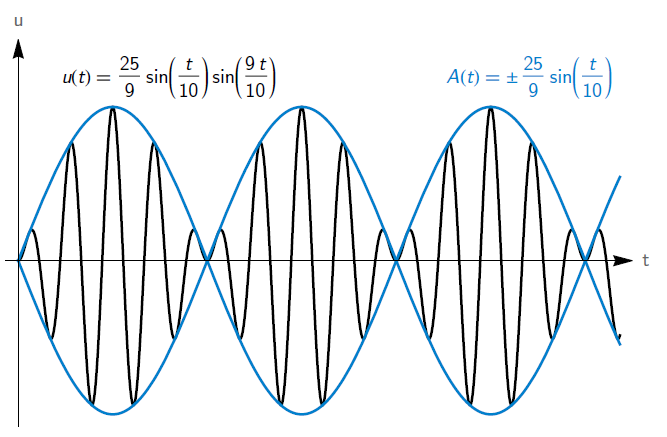
\includegraphics[width=10cm]{AN0.png}
\end{figure}

\end{block}
\end{frame}

\begin{frame}

$$y(t)=(A+x(t))\cos(\omega_ct+\theta_c),\hspace{3mm} A>|x(t)|_{\max}$$
\begin{figure}[h]
    \centering
    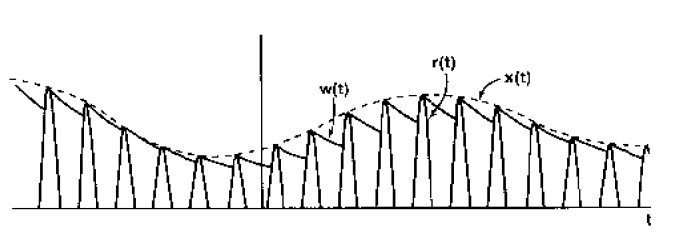
\includegraphics[width=10cm]{AM.png}
\end{figure}
\end{frame}


\begin{frame}
\frametitle{Complex Analysis}
We say that a function $f : \mathbb{C}\rightarrow\mathbb{C}$ is complex
differentiable, or holomorphic, at $z \in\mathbb{C}$ if
$$f'(z):=\lim_{h\rightarrow0\atop h\in\mathbb{C}}\dfrac{f(z+h)-f(z)}{h}$$
exists.
\begin{block}{}
We say that a function is holomorphic on an open set $\Omega\subset \mathbb{C}$ if it is holomorphic at every $z \in \Omega$. A function that is holomorphic on $\mathbb{C}$ is called entire.
\end{block}

\end{frame}

\begin{frame}
\begin{block}{Some Properties}
\begin{enumerate}
\item A holomorphic function is automatically infinitely often differentiable;
\item A holomorphic function is automatically analytic (has a power series
expansion);
\item Any closed curve integral of a holomorphic function is vanishes.
\end{enumerate}
\end{block}

\end{frame}

\begin{frame}
\begin{block}{The Cauchy-Riemann Differential Equations}
For a complex function
$$f:\mathbb{C}\rightarrow\mathbb{C},\hspace{3mm}f(x+iy)=u(x,y)+iv(x,y)$$
where $u,v:\mathbb{R}^2\rightarrow\mathbb{R}$, if $f$ is complex differentiable, then
$$\dfrac{\partial u}{\partial x}=\dfrac{\partial v}{\partial y},\hspace{3mm}\dfrac{\partial u}{\partial y}=-\dfrac{\partial v}{\partial x}$$

\end{block}

\end{frame}

\begin{frame}
\begin{block}{}
Define differential operators
$$\dfrac{\partial }{\partial z}=\dfrac{1}{2}\Big(\dfrac{\partial }{\partial x}+\dfrac{1}{i}\dfrac{\partial }{\partial y}\Big),\hspace{3mm}\dfrac{\partial }{\partial \overline{z}}=\dfrac{1}{2}\Big(\dfrac{\partial }{\partial x}-\dfrac{1}{i}\dfrac{\partial }{\partial y}\Big)$$
For holomorphic function,
$$f'(z)=\dfrac{\partial f}{\partial z}=2\dfrac{\partial u}{\partial z},\hspace{3mm} \dfrac{\partial f}{\partial \overline{z}}=0$$
Suppose that the partial derivatives of $u$ and $v$ exist, are continuous and satisfy the Cauchy-Riemann equations. Then $f$ is holomorphic.
\end{block}
\end{frame}

\begin{frame}
\begin{block}{Sets in the Complex Plane}
\begin{enumerate}
\item A set $\Omega\subset\mathbb{C} $ is called open if for every $z\in\Omega$ there exists an $\varepsilon>0$ such that $B_{\varepsilon}(z)=\lbrace w\in\mathbb{C}:|w-z|<\varepsilon\rbrace\subset\Omega$. A set is called closed if its complement is open.
\item A set $\Omega\subset\mathbb{C}$ is called bounded if $\Omega\subset B_R(0)$ for some $R>0$.
\item A set $K\subset\mathbb{C}$ is called compact if every sequence in $K$ has a subsequence that converges in $K$. A set $K\in\mathbb{C}$ is compact if and only if it is closed and bounded.
\item An open (closed) set $\Omega\subset\mathbb{C}$ is called disconnected if there exist two open (closed) sets $\Omega_1,\Omega_2\subset\mathbb{C}$ such that $\Omega_1\cap\Omega_2=\emptyset$ and $\Omega=\Omega_1\cup\Omega_2$. If $\Omega$ is not disconnected, $\Omega$ is called connected. A set $\Omega\subset\mathbb{C}$ is conneted if and only if for any two points in $\Omega$ there exists a curve joining them.
\item A \textcolor[rgb]{0,0.6,0.3}{\textit{region}} or \textcolor[rgb]{0,0.6,0.3}{\textit{domain}} in $\mathbb{C}$ is an open and conneted set.
\end{enumerate}
\end{block}
\end{frame}

\begin{frame}
\begin{block}{}
We define the diameter of a set $\Omega\subset\mathbb{C}$ by
$$\text{diam}(\Omega)=\sup_{z,w\in\Omega}|z-w|$$
If $(\Omega_n)$ is a sequence of non-empty compact sets such that $\Omega_{n+1}\subset\Omega_n$ for $n\in\mathbb{N}$ and diam $\Omega_n\rightarrow0$ as $n\rightarrow\infty$, then there exists a unique point $w\in\mathbb{C}$ such that $w\in\Omega_n$ for all $n$.
\end{block}
\end{frame}

\begin{frame}
\begin{block}{Power Series}
For a power series
$$f(z)=\sum\limits_{n=0}^{\infty}a_nz^n$$
it defines a holomorphic function in its disc of convergence. The (complex) derivative of $f$ is also a power series obtained by differentiating term by term the series for $f$, that is 
$$f'(z)=\sum\limits_{n=1}^{\infty}na_nz^{n-1}$$
and $f'$ has the same radius of convergence as $f$.
\end{block}
\begin{block}{}
A power series is infinitely complex differentiable in its disc of convergence, and the higher derivatives are also power series obtained by termwise differentiation.
\end{block}
\end{frame}

\begin{frame}
\begin{block}{Analytic Function}
A function $f$ defined on an open set $\Omega\subset\mathbb{C}$ is said to be analytic (or have a power series expansion) at a point $z_0\in\Omega$ if there exists a power series $\sum\limits_{n=0}^{\infty}a_n(z-z_0)^n$ centered at $z_0$, with positive radius of convergence, such that
$$f(z)=\sum\limits_{n=0}^{\infty}a_n(z-z_0)^n$$
for all $z$ in a neighborhood of $z_0$. If $f$ has a power series expansion at every point in $\Omega$, we say that $f$ is analytic on $\Omega$.
\end{block}
\end{frame}

\begin{frame}
\begin{block}{Integrals along Complex Curves}
Let $\Omega\subset\mathbb{C}$ be an open set, $f$ holomorphic on $\Omega$ and $\mathcal{C}^*\subset\Omega$ an oriented smooth curve. We then define the integral of $f$ along $\mathcal{C}^* $ by 
$$\int_{\mathcal{C}^*}f(z)dz=\int_If(\gamma(t))\cdot\gamma'(t)dt$$
where $\gamma:I\rightarrow \mathcal{C}^* $ is a parametrization of the parameterized curve $\mathcal{C}^*$.
\end{block}
\begin{block}{Curve Length}
$$\ell(\mathcal{C})=\Bigg|\int_{\mathcal{C}}dz\Bigg|$$
$$\int_{-\mathcal{C}^*}f(z)dz=-\int_{\mathcal{C}^*}f(z)dz,\hspace{3mm}\Bigg|\int_{\mathcal{C}^*}f(z)dz\Bigg|\leqslant\ell(\mathcal{C})\cdot\sup_{z\in\mathcal{C}}|f(z)|$$
\end{block}
\end{frame}

\begin{frame}
\begin{block}{Primitive}
Let $\Omega\subset\mathbb{C}$ be an open set, $f:\Omega\rightarrow\mathbb{C}$. A primitive for $f$ is a holomorphic function $F:\Omega\rightarrow\mathbb{C}$ such that $f(z)=F'(z)$ for all $z\in\Omega$.
\end{block}

\begin{block}{}
If a continuous function $f$ has a primitive $F$ in $\Omega$, and $\mathcal{C}^*$ is a curve in $\Omega$ that begins at $w_1$ and ends at $w_2$, then
$$\int_{\mathcal{C}^*}f(z)dz=F(w_2)-F(w_1)$$
Especially, if $\mathcal{C}^*$ is a closed curve, 
$$\int_{\mathcal{C}^*}f(z)dz=0$$
If $f$ is holomorphic in a region $\Omega$ and $f'=0$, then $f$ is constant.
\end{block}
\end{frame}

\begin{frame}
\begin{block}{Goursat's Theorem}
Let $\Omega\subset\mathbb{C}$ be an open and $f$ \textcolor[rgb]{0,0.6,0.3}{\textit{holomorphic}} on $\Omega$. Let $T\subset\Omega$ be a \textcolor[rgb]{0,0.6,0.3}{\textit{triangle}} whose interior is also contained in $\Omega$. Then
$$\oint_Tf(z)dz=0$$
and therefore, for a \textcolor[rgb]{0,0.6,0.3}{\textit{rectangle}} $R$,
$$\oint_Rf(z)dz=0$$
\end{block}
\end{frame}

\begin{frame}
\begin{block}{Morera's Theorem}
Let $\Omega\subset\mathbb{C}$ be an open, connected set and let $f : \Omega \rightarrow \mathbb{C}$ be continuous. Suppose that 
$$\oint_Tf(z) dz = 0\hspace{3mm} \text{for any triangle \textit{T} wholly contained in }\Omega$$
\begin{enumerate}
\item $f$ has a primitive on $\Omega$
\item ($f$ is holomorphic.) 
\end{enumerate}
\end{block}
\begin{block}{Local Existence of Primitives}
A holomorphic function in an open disc has a primitive in that disc.
\end{block}
\end{frame}

\begin{frame}
\begin{block}{Proof}
$\forall z\in\Omega$, choose some $z_0$ such that $z\in B_{\delta}(z_0)$ for some $\delta>0$. Then define the function
$$F:B_{\delta}(z_0)\rightarrow\mathbb{C},\hspace{3mm}F(z)=\int_{\mathcal{C}(z_0,z)}f(\zeta)d\zeta$$
where $\mathcal{C}(z_0,z)$ is parametrized by 
$$\gamma:[0,1]\rightarrow\mathbb{C},\hspace{3mm}\gamma(t):=(1-t)z_0+tz$$

Suppose that $z+h\in B_{\delta}(z_0)$ for some $h$. Any integral along the triangle with vertices $z_0,z$ and $z+h$ vanishes, so that
\begin{align*}
F(z+h)-F(z)&=\int_{\mathcal{C}(z,z+h)}f(\zeta)d\zeta=\int_0^1f((1-t)z+t(z+h))\cdot hdt\\
&=h\int_0^1f(z+th)dt
\end{align*}
\end{block}
\end{frame}

\begin{frame}
\begin{block}{Proof (continued)}
Since $f$ is continuous, $f(z+th)=f(z)+o(h)$ as $h\rightarrow0$, so
$$F(z+h)=F(z)+hf(z)+o(h)$$
\end{block}
\end{frame}

\begin{frame}
\begin{block}{Cauchy's Theorem for a Disc}
If $f$ is holomorphic in a disc, then
$$\oint_{\mathcal{C}}f(z)dz=0$$
for any closed curve $\mathcal{C}$ in that disc.
\end{block}
\begin{block}{Cauchy's Theorem}
Suppose $f$ is holomorphic in an open set $\Omega\subset\mathbb{C}$ containing a circle $C$ and its interior. Then
$$\oint_Cf(z)dz=0$$
Cauchy's theorem holds for other contours, as long as any point $z$ in their interior can be joined to some selected $z_0$ (connected) through straight lines.
\end{block}
\end{frame}

\begin{frame}
\begin{block}{Evaluation of Real Integrals using Cauchy's Theorem}
\begin{figure}[h]
    \centering
    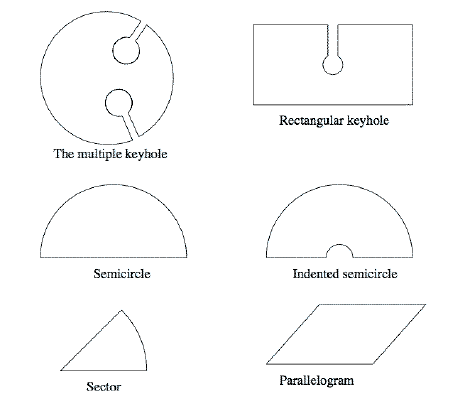
\includegraphics[height=7cm]{toy.png}
\end{figure}
\end{block}
\end{frame}

\begin{frame}
\begin{block}{Jordan's Lemma}
Assume that for some $R_0>0$ the function $g:\mathbb{C}\setminus B_{R_0}(0)\rightarrow\mathbb{C}$ is holomorphic. Let
$$f(z)=e^{iaz}g(z),\hspace{3mm}\text{for some }a>0$$
Let
$$C_R=\lbrace z\in\mathbb{C}:z=R\cdot e^{i\theta},0\leqslant\theta\leqslant\pi\rbrace$$
be a semi-circle segement in the upper half-plane and assume that
$$\sup_{0\leqslant\theta\leqslant\pi}|g(Re^{i\theta})|\xlongrightarrow{R\rightarrow\infty}0$$
Then
$$\lim_{R\rightarrow \infty}\int_{C_R}f(z)dz=0$$
 
\end{block}
\end{frame}

\begin{frame}
\begin{block}{Cauchy Integral Formulas}
Suppose $f$ is a holomorphic function in an open set $\Omega\subset\mathbb{C}$. If $D$ is an open disc whose closure is contained in $\Omega$ then
$$f(z)=\dfrac{1}{2\pi i}\oint_C\dfrac{f(\zeta)}{\zeta-z}d\zeta$$
where $C=\partial D$ is the (positively oriented) boundary circle of $D$. (It holds for all toy contours.)

\end{block}
\begin{block}{}
If $f$ is a holomorphic function in an open set $\Omega\subset\mathbb{C}$, then $f$ has infinitely many complex derivatives in $\Omega$. Moreover, if $D$ is an open disc whose closure is contained in $\Omega$,
$$f^{(n)}=\dfrac{n!}{2\pi i}\oint_C\dfrac{f(\zeta)}{(\zeta-z)^{n+1}}$$
where $C=\partial D$ is the (positively oriented) boundary circle of $D$.
\end{block}
\end{frame}

\begin{frame}
\begin{block}{Holomorphic Functions are Analytic}
Suppose $f$ is a holomorphic function in an open set $\Omega$. If $D$ is an open disc centered at $z_0$ whose closure is contained in $\Omega$, then $f$ has a power series expansion at $z_0$
$$f(z)=\sum\limits_{n=0}^{\infty}a_n(z-z_0)^n$$
for all $z\in D$ and the coefficients are given by
$$a_n=\dfrac{f^{(n)}(z_0)}{n!},\hspace{3mm}n\in\mathbb{N}$$
\end{block}
\end{frame}


\begin{frame}
\begin{block}{Uniqueness of Holomorphic Functions}
Let $\Omega\subset\mathbb{C}$ be a region and $f,g:\Omega\rightarrow\mathbb{C}$ two holomorphic functions. Suppose that $S\subset\Omega$ has an accumulation point that is contained in $\Omega$ and that
$$f(z)=g(z)\hspace{3mm}\text{for all }z\in S$$
Then $f(z)=g(z)$ for all $z\in\Omega$.
\end{block}
\begin{block}{Analytic Continuation}
Let $M\subset\mathbb{C}$ be a any set and $f:M\rightarrow\mathbb{C}$ any function. Let $\Omega$ be a region with $M\subset\Omega$ and $g:\Omega\rightarrow\mathbb{C}$ a holomorphic function such that $g(z)=f(z)$ for $z\in M$. Then $g$ is called an analytic continuation of $f$ to $\Omega$.
\end{block}
\end{frame}

\begin{frame}
\begin{block}{Singularities}
Let $\Omega\subset\mathbb{C}$ be open, $z_0\in\Omega$ and $f:\Omega\setminus\lbrace z_0\rbrace\rightarrow\mathbb{C}$ holomorphic. Then $f$ is said to have a point singularity or isolated singularity at $z_0$.
\begin{enumerate}
\item The singularity is said to be removable if there exists an analytic continuation $\tilde{f}:\Omega\rightarrow\mathbb{C}$. (such $\tilde{f} $ is unique)
\item The singularity is said to be a \textcolor[rgb]{0,0.6,0.3}{\textit{pole}} if $g=1/f$ is holomorphic on $\Omega\setminus\lbrace z_0\rbrace$ and has a removable singularity at $z_0$ such that the analytic continuation $\tilde{g}$ of $g$ satisfies $\tilde{g}(z_0)=0$.
\item The singularity is said to be essential if it is neither removable nor a pole.
\end{enumerate}
\end{block}
\end{frame}

\begin{frame}
\frametitle{Residue}
Let $\Omega\subset\mathbb{C}$ be a domain and $f:\Omega\setminus\lbrace z_0\rbrace\rightarrow\mathbb{C}$ have a pole of order $n$ at $z_0$. Then
$$\text{res}_{z_0}f=\dfrac{1}{(n-1)!}\lim_{z\rightarrow z_0}\dfrac{d^{n-1}}{dz^{n-1}}\big((z-z_0)^nf(z)\big)$$ 

\begin{block}{Residue Theorem}
Suppose that $f$ is holomorphic in an open set containing a (positively oriented) toy contour $\mathcal{C}$ and its interior, except for poles at the points $z_1,\cdots,z_N$ inside $\mathcal{C}$. Then
$$\int_{\mathcal{C}}f(z)dz=2\pi i\sum\limits_{k=1}^N\text{res}_{z_k}f$$
\end{block}

\end{frame}

\begin{frame}
\begin{block}{Complex Logarithm}
On any simply connected open set $\Omega$, $(1\in\Omega,0\notin\Omega)$, set
$$\ln 1=0,\hspace{3mm}\ln z=\int_{\mathcal{C}}\dfrac{dz}{z}$$
where $\mathcal{C}\subset\Omega$ is any simple curve joining $1\in\Omega$ to $z\in\Omega$.
\begin{enumerate}
\item $\ln(re^{i\phi})=\ln r+\varphi i, (r>0,-\pi<\phi<\pi)$
\item $\ln(re^{i\phi})=\ln r+\varphi i, (r>0,0<\phi<2\pi)$
\end{enumerate}
\end{block}
\end{frame}

\begin{frame}
\begin{block}{Complex Powers}
$$z^{\alpha}=e^{\alpha\ln z},\hspace{3mm}\alpha\in\mathbb{C},z\in\mathbb{C}\setminus\mathbb{R}_-^0$$
\end{block}
\begin{block}{Complex Roots}
$$\sqrt[n]{\alpha}=z^{1/n}$$
\end{block}
\end{frame}

\begin{frame}
\begin{block}{Residue Calculus for Functions with Branch Points}
Let $P$ and $Q$ be polynomials of degree $m$ and $n$, respectively, where $n\geqslant m+2$. If $Q(x)\neq0$ for $x>0$, if $Q$ has a zero of order at most 1 at the origin and if
$$f(z)=\dfrac{z^{\alpha}P(z)}{Q(z)},\hspace{3mm}0<\alpha<1$$
then
$$\text{p.v.}\int_0^{\infty}\dfrac{x^{\alpha}P(x)}{Q(x)}dx=\dfrac{2\pi i}{1-e^{2\pi \alpha i}}\sum\limits_{j=1}^k\text{res}_{z_j}f$$
\end{block}
\end{frame}

\begin{frame}
\frametitle{The (Unilateral) Lapalace Transform}
Let $f:[0,\infty)\rightarrow\mathbb{R}$ be a continuous function such that
$$\sup_{t\in[0,\infty)}e^{-\beta t}|f(t)|<\infty\hspace{3mm}\text{for some }\beta\geqslant0$$
Then the function $F:(\beta,\infty)\rightarrow\mathbb{R}$,
$$F(p)=(\mathscr{L} f)(p)=\int_0^{\infty}e^{-pt}f(t)dt$$
is called the Lapalace transform of $f$.

\begin{align*}
(\mathscr{L}f')(p)&=\int_0^{\infty}e^{-pt}f'(t)dt=\int_0^{\infty}pe^{-pt}f(t)dt-f(0)\\
&=p\cdot(\mathscr{L}f)(p)-f(0)\\
(\mathscr{L}f'')(p)&=p^2(\mathscr{L}f)(p)-p\cdot f(0)-f'(0)
\end{align*}
\end{frame}
\begin{frame}
\begin{block}{The Bromwich Integral}
Let $\Omega \subset \mathbb{C}$ be an open set, $\beta\in \mathbb{R}$ and $F :\Omega \rightarrow\mathbb{C}$ analytic for all $z \in \mathbb{C}$ with $\text{Re} z \geqslant\beta$. Then the Bromwich integral of $F$ is
$$(\mathscr{M}F)(t) =\dfrac{1}{2\pi i}\int_{\mathcal{C}^*}e^{pt}F(p) dp=\dfrac{1}{2\pi i}\int_{\beta-i\infty}^{\beta+i\infty}e^{pt}F(p) dp$$
\begin{enumerate}
\item For $t > 0$, the Bromwich integral $\mathscr{M}F(t)$ is usually calculated by closing the contour on the left and applying the residue theorem.
\item For $t < 0$ we close the contour on the right.
\end{enumerate}
\end{block}
\begin{block}{Convolution}
$$(f * g)(t) :=\int^t_0f (t-s)g(s) ds,\hspace{3mm}(\mathscr{L})(f*g)=(\mathscr{L}f)\cdot(\mathscr{L} g)$$
\end{block}
\end{frame}

\begin{frame}
\begin{figure}[h]
    \centering
    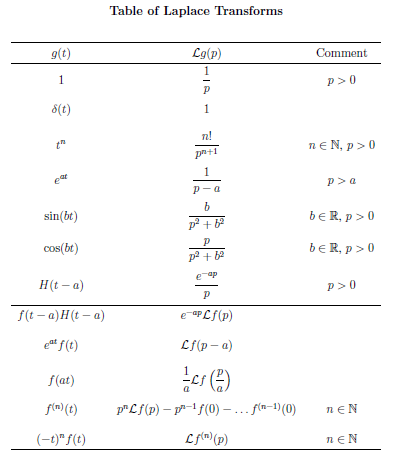
\includegraphics[height=8.2cm]{lapalace.png}
\end{figure}
\end{frame}

\begin{frame}
\frametitle{The Fourier Transform}
\begin{block}{}
$$\widehat{f}(\xi)=\dfrac{1}{\sqrt{2\pi}}\int_{-\infty}^{\infty}f(x)e^{-i\xi x}dx$$
$$\widehat{(f')}(\xi)=i\xi\cdot\widehat{f}(\xi)$$
$$\dfrac{d}{d\xi}\widehat{f}(\xi)=\widehat{(-ix)f}(\xi)$$
\end{block}
\end{frame}
\end{document}
